%!TEX root = thesis.tex

\chapter{Introduction}
\label{ch:intro}

\section{The Human-Computer Interface}


Human-Computer Interaction  (HCI) is slow. The information per minute rate is still low nowadays, and innovation is progressing slowly. Since the introduction of the mouse in the seventies no revolutionary new peripherals where introduced that aid the communication with a computer. 

New and revolutionary ideas are required to create new perhiperials that improve productivity, but are still intuitive and thus easy to learn to use. To get inspiration for improvement, one can look around and study already existing 'solutions', for example inter human communication. 

When two people are in a room and don't have a audio or visual limitation, they will probably communicate by speech. But there is much more going on than only producing and interpreting words. The intonation, speed and other small variations in the voice add a lot more information to the words. But also the facial expression and body language give more space for expression. Some people like to 'talk with their hands' while telling a story, something that adds more expression to the transmitted information.


\section{Sign Language}

A deaf person can't interpret spoken words, at least not by listening. He or she is highly depended on visual information. Sign languages have been created or invented to aid this visual communication. In these languages two elements have an important role, the face and the hands. These body parts give the most expressive power. The face because it is very good for expressing feelings and emotions, and the hands because they are very flexible and morphable. The hands are especially interesting because there are countless combinations of finger poses and orientations. 

Speech generation, speech recognition, facial expression recognition and sign language interpretation have all been studied before. Research has been done in automated sign language interpretation using computer vision\cite{Buehler2009}\cite{RichardBowden2004}. The problem with interpreting sign language is a very large vocabulary, segmentation of the different gestures and representing the gestures in a robust way.

\section{Goal and motivation}
\label{sec:goal}
The goal of this thesis is to describe the design, build and evaluation process of a system for hand pose recognition. The system needs to be fast and user friendly. 

\begin{itemize}
	\item Real time performance (between 10 and 50 fps)
	\item Normal consumer processing power
	\item Normal RGB camera (webcam)
	\item No gloves or skin mounted electromechanical sensors
	\item No calibration or initialization
	\item Minimal configuration/parameters
\end{itemize}
	

To realize these requirements some restrictions on the system's setting are required:
\begin{itemize}
	\item One person in the image
	\item Person is wearing clothing with long sleeves
	\item Good enough lightning conditions
	\item No skin like colors in the image.
\end{itemize}

The system can be used to increase the HCI speed, but also introduce the possibility to add more feeling and detail to Human-Computer Interaction, especially for real time interaction. Using hand poses for Computer aided music composing is interesting but challenging, since the realtime element plays an important role. Also, in a live performance setting, it is much more interesting to look at somebody using his body to interact with a machine than only click of a mouse.


\section{Solfege, The Curwen Hand symbols}


For this experiment Sonic Gesture is trained with the Curwen Solfege set\cite{choksy1999}.


\begin{figure}[htbp]
	\center{}
	\label{fig:curwen}
	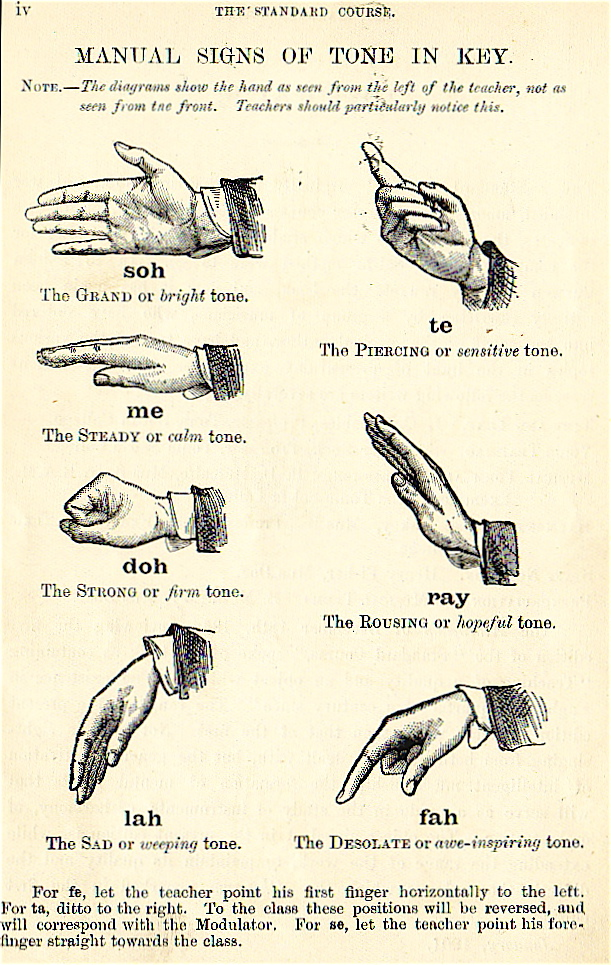
\includegraphics[width=0.3\linewidth]{figures/curwen.jpg}
	\caption{Curwen Hand Symbols}
\end{figure}

\begin{figure}[htbp]
	\center{}
	\label{fig:doremifa}
	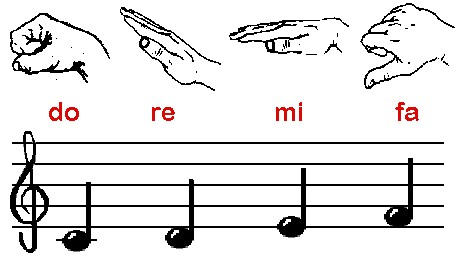
\includegraphics[width=0.3\linewidth]{figures/doremifa.jpg}
	\caption{Do Re Mi Fa}
\end{figure}

\begin{figure}[htbp]
	\center{}
	\label{fig:solatido}
	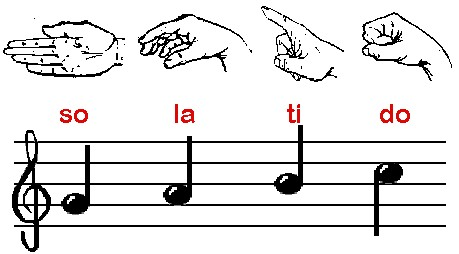
\includegraphics[width=0.3\linewidth]{figures/solatido.jpg}
	\caption{Sol La Ti Do}
\end{figure}

\begin{figure}[htbp]
	\center{}
	\label{fig:guidonian}
	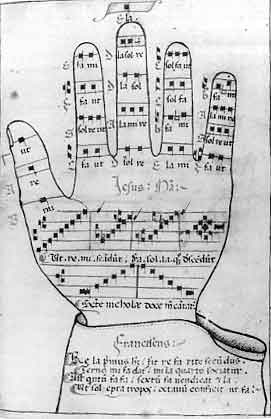
\includegraphics[width=0.3\linewidth]{figures/guidonian_hand.jpg}
	\caption{Guidonian Hand}
\end{figure}


\section{Related Work}
\cite{Erol2007} gives a good overview of the current state and limitations of computer vision based hand pose and gesture recognition.



